
\chapter{Research Overview}\label{sc:research}

The research in this thesis is presented in seven papers. 
Fig. \ref{fig:papers} shows how the papers are related. Papers 1, 2,
4, 5 and 6 are published works, while
3 and 7 are submitted for publication. The format of all papers have been
modified to suit this thesis. The references for each paper has been
included into the complete reference list at the end of the
thesis. The content of papers 1, 2, 4, 5 and 6 have
not been modified in any way from the published version.

The topic of the research is efficient ADCs in
nano-scale CMOS technology. We focus on two separate paths:
\begin{enumerate}
\item Assume switched-capacitor implementation challenges will be
  solved and investigate ADCs with sigma-delta modulator front-end and pipelined back-end.
\item Investigate efficient circuit solutions for pipelined ADCs

\end{enumerate}
The first path include papers 1, 2 and 3 while the second path
include papers 4, 5, 6 and 7. We will describe the two paths separately.

\begin{figure}[htbp]
\centerline{ 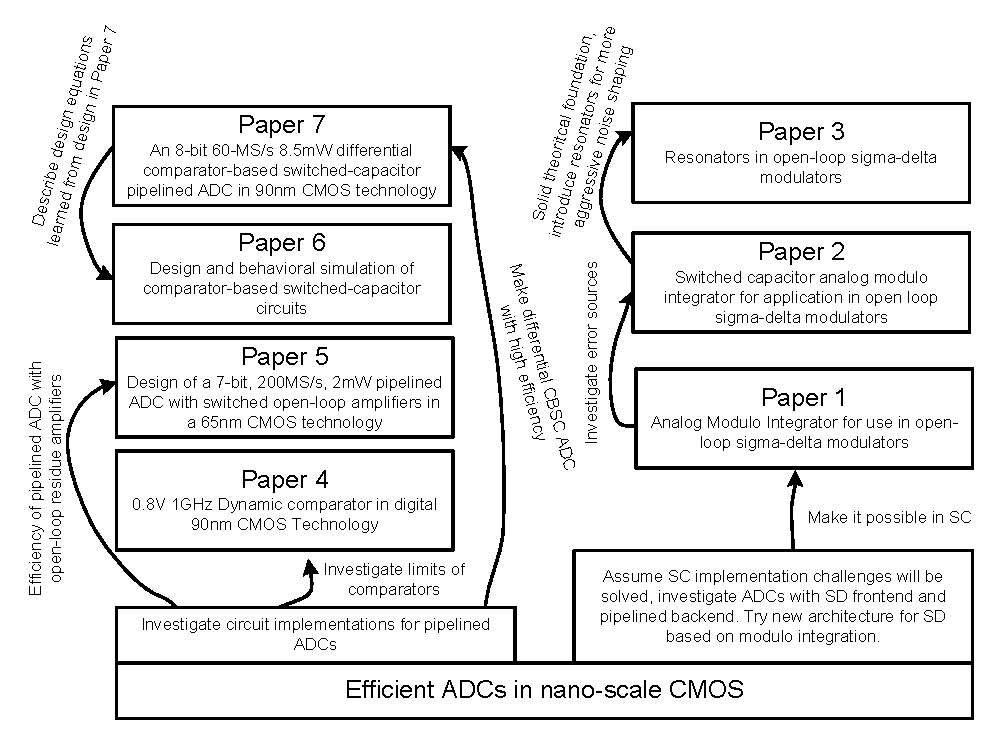
\includegraphics[width=\myfigwidthm]{graphics/paperrel}}
  \caption{How papers relate to each other and the central theme}
  \label{fig:papers}
\end{figure}

%\newpage

\section{Open-loop sigma-delta modulators (OLSDM)}
The open-loop sigma-delta
modulators in this thesis brings the OLSDM architecture to
switched-capacitor architectures. Our motivation for creating an OLSDM
is the use in hybrid converters. The idea is to use an OLSDM front-end and pipelined ADC
back-end. Such hybrid converters can achieve good performance
\cite{brooks97}. 
Previous OLSDM architectures have been digital-to-analog
modulators \cite{wisland03a}, or frequency sigma-delta modulators \cite{hovin97}. 

%Paper 1 introduce the
%switched-capacitor modulo integrator and how it could be used in an
%OLSDM. In paper 2, which is an invited paper based on paper 1, we go
%into detail on some of the error sources in OLSDM and how they can be
%corrected for. 

%Paper 3 place the theory of OLSDM on a solid ground
%by deriving conditions for when an OLSDM is equivalent to a
%sigma-delta modulator. It also introduces the modulo resonator, and
%shows an example of a 13-bit ENOB modulator with an OSR of
%4. 

Fig. \ref{fig:olsdmvspipe} shows an example of why we believe an
OLSDM-Pipelined hybrid might have an efficiency advantage. The figure
shows a comparison between a 14-bit pipelined ADC and a 14-bit hybrid
ADC.
A 14-bit pipelined ADC need
a sample and hold  and seven 1.5-bit stages\footnote{The
  number of stages can be reduced if more bits are
converted in each stage. This requires more comparators in each stage,
a 1.5-bit pipelined stage has two comparators. The accuracy of a
comparator in a B-bit stage must be $\pm V_{REF}/2^B$. Mismatch determine
the accuracy of the comparators, which usually limit the number of bits per
stage to 3-bits.} if we use a 7-bit back-end ADC. 
The hybrid converter has 5 stages before the back-end (no sample an hold), a saving of three
stages. The hybrid has two modulo resonators and a modulo integrator
that result in a fifth order noise transfer function.

To clarify why we believe that OLSDM can have an advantage, we will
describe some of the challenges in high-speed, high-accuracy
converters. These are:

\begin{description}
\item[Clock skew]  In pipelined ADCs clock skew between  the sub-ADCs and the
  sampling network (input switches and sampling capacitors) is a challenge. This skew (difference in delay) cause a signal dependent
  offset. The problem can be alleviated by placing a sample and hold
  before the first stage.

In the hybrid only the sampling capacitors are connected to the
input. Thus, clock skew is not a problem and the
hybrid does not need a separate sample and hold. 


\item[Capacitor size] In a 14-bit pipelined converter with low signal swing
 the capacitor size can be large. For 1V peak-to-peak input swing the
  input capacitance has to be 53pF (from \req{cap}). In 90nm CMOS this
  capacitance will measure 163$\mu$m by 163$\mu$m, which is a large
  area. 

The
  capacitor size can be reduced by oversampling.
  In the hybrid example in Paper 3 the oversampling ratio is four, accordingly the
  sampling capacitors can be reduced by a factor of four (13pF). 

\item[Opamp DC gain] is a significant challenge, and it is equivalent in
  the hybrid and pipelined ADC. The
error introduced by finite opamp gain cause static 
non-linearities in a pipelined ADC|this limits the accuracy of the
converter to
below the gain of the first opamp.

 In the hybrid the
finite opamp
gain
cause leakage of quantization error from each modulo integrator. The error is
shaped by the preceding signal transfer function. As a result, the
opamp gain can be scaled differently than in a pipelined ADC. 

%\item[Capacitor mismatch] is a challenge that is the same in the two
%  architectures. 

\item[ADC speed] translate into opamp branch current. The hybrid runs four
  times faster than the pipelined ADC, but has four times less
  capacitance, which cancel  with respect to current consumption. But the hybrid has a
  switched-capacitor circuit with at least three clock phases, compared to
  two clock phases for pipelined ADC. Assuming the settling requirements are
  the same for the pipelined ADC and the hybrid, the hybrid opamps must be 1.5 times faster than in the
  pipelined ADC. Preliminary simulations suggest that the hybrid will
  require opamps even faster than this, but a thorough study
  is left for future work.
\end{description}


\begin{figure}[htbp]
\centerline{ 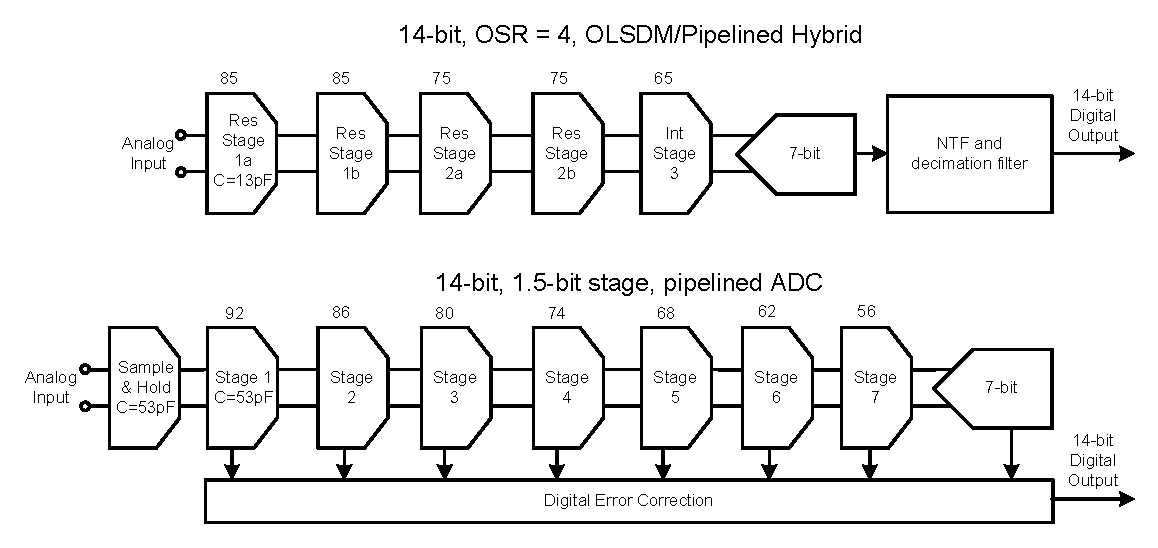
\includegraphics[width=\myfigwidthm]{graphics/olsdmvspipe}}
  \caption{Comparison between a 14-bit high-speed OLSDM and a 14-bit
    pipelined converter. The numbers above the stages denote the
    required operational amplifier
    DC gain in dB.}
  \label{fig:olsdmvspipe}
\end{figure}


\subsubsection{Paper 1: Analog Modulo Integrator For Use In Open-Loop Sigma-Delta
  Modulators}

In this paper we introduce the switched-capacitor modulo
integrator. The modulo integrator makes it possible to design an
open-loop sigma-delta modulator. The theory of OLSDM and
analog modulo integration is explained and verified through simulation.


\subsubsection{Paper 2: Switched Capacitor Analog Modulo Integrator For Application
  In Open Loop Sigma-Delta Modulators}
Paper 2 is an invited paper based on Paper 1, hence there is some
overlap in the areas covered. Paper 2 discuss one of the error effects
in OLSDM (false modulo) and investigate effects of a non-linear
quantizer.
Behavioral level simulations in SPICE of the analog modulo
integrator verify the function, and prove the concept of
amplitude modulated OLSDM.




\subsubsection{Paper 3: Resonators In Open-Loop Sigma-Delta Modulators}

In  Paper 3 we introduce the modulo resonator for 
use in open-loop sigma-delta modulators. The OLSDM 
presented in this work is intended for use in high accuracy (14- 
bit), high-speed ADCs. 
The modulo resonator is used with a modulo notch filter 
to insert a zero in the noise transfer function at a non-zero 
frequency. 
The effect of finite gain in modulo integrators and modulo 
resonators are described and verified through simulation. 
The modulo resonator and previously published modulo integrator are
used in a behavioral model of a switched-capacitor  
fifth-order OLSDM with more than 13-bit effective number of 
bits for an oversampling ratio of four.

 We prove for the N-order 
OLSDM that the number of bits in the quantizer (B) must be 
larger than N to ensure equivalence between OLSDM and sigma-delta modulation. 



%\newpage
\section{Efficient circuit solutions for pipelined ADCs}
%The pipelined ADC architecture is a popular ADC architecture  for 8-bit to 15-bit converters with speeds
%from 10MS/s to 1GS/s.
Circuit solutions that remove the opamp from switched-capacitor
circuits have received interest from the research community. The idea
is to replace the hard to make opamps with something more amenable to
nano-scale CMOS integration. In the papers we have focused on two
techniques; open-loop amplifiers, and comparator-based switched
capacitor circuits. Not only are these techniques more amenable to
nano-scale integration, but CBSC has been shown to have a fundamental
efficiency advantage over opamp based integration \cite{lee08}. 

We have also investigated the
comparators used in the sub-ADC in the pipelined ADCs.

% Paper 4 investigates a comparator for the sub-ADC in a pipelined ADC
% and its limitations in nano-scale CMOS. Paper 5 use open-loop
% residue amplifiers in a design of a 7-bit pipelined ADC. 
% Paper 6 introduce design equations for comparator based
% switched-capacitor circuits.
% Paper 7 is the first implementation of a differential
% comparator-based switched capacitor (CBSC) pipelined ADC.  CBSC has a
% fundamental efficiency advantage over opamp-based 
% pipelined ADC, as was shown in Chapter \ref{sc:limits} and
% \cite{lee08}.


\subsubsection{Paper 4:  0.8V 1GHz Dynamic Comparator In Digital 90nm CMOS
  Technology}

This paper present simulations of a dynamic comparator in 90nm CMOS
technology. It
shows how 90nm CMOS technology can achieve high speed at low supply
voltages. 

One of the challenges in dynamic comparators is controlling
the offset over process corners. As the signal swing scales down (due
to supply voltage scaling) the demands on comparators in pipelined ADC
become harder to fulfill, but as the paper shows, at 90nm CMOS it is
quite possible to have high-speed and low supply voltage. 



\subsubsection{Paper 5: Design of a 7-bit 200MS/s, 2mW Pipelined ADC With Switched
  Open-Loop Amplifiers In a 65nm CMOS Technology}

In this paper we present the design of a
7-bit 200MS/s pipelined ADC with switched open-loop amplifiers in a
65nm CMOS technology. As a
result of turning
off the open-loop amplifiers during sampling we reduce the power
dissipation by 23\%. The ADC achieves a SNDR
of 40dB close to the Nyquist frequency, with a power dissipation of
2mW, which results in a 
Walden FOM of 0.13pJ/step and a Thermal FOM of 1.6fJ/step.

%This FOM is good compared to other converters. The paper proves that low resolution converters can be
%efficiently designed as pipelined ADCs. 

%At ISSCC 2008 a analog-to-digital converter
%was presented that eclipsed the performance of any previous low
%resolution ADC
%\cite{vanderplas08} (7-bit 150MS/s 0.133 $\mu$W). But the
%architecture requires $2^{B-1}$ comparators, and they must all have $B$
%bit resolution. Hence, the architecture is unsuited for higher
%resolution.
\subsubsection{Paper 6: Design and Behavioral Simulation of Comparator-Based Switched
  Capacitor Circuits}
This paper summarize some of the design equations derived in designing
and debugging the chip in Paper 7. It presents a method for
calculating the required 
parameters for 
comparator-based switched capacitor circuits. The parameters are
capacitance ($C$), current ($I_0$), comparator delay ($T_D$), current
source output resistance ($R_o$) and comparator threshold 
($V_{ct}$). The design equations
are verified with behavioral simulations in SPICE and MATLAB.

\subsubsection{Paper 7: An 8-bit 60-MS/s 8.5mW Differential Comparator-Based Switched-Capacitor
  Pipelined ADC in 90nm CMOS Technology}
In this paper we present the first differential comparator-based switched-capacitor (CBSC) pipelined ADC. The switched-capacitor multiplying
digital-to-analog converter (MDAC)
use current sources and a comparator to do charge transfer. Continuous
time bootstrapped switches are used in the first stage to reduce signal dependent switch
resistance. A simple calibration algorithm correct for
comparator delay variation caused by the manufacturing process. Calibration reduces
ramp overshoot, which dominate the non-linearity in CBSC ADCs. The ADC is produced in a 90nm
low-power CMOS technology. The ADC core is 0.85mm x 0.35mm, with a
1.2V supply for the core and 1.8V for input switches. The ADC
has an effective number of bits (ENOB) of 7.05-bit, and a power
dissipation of 8.5mW at 60MS/s. The ADC achieves an Waldon FOM of
1.07pJ/step and Thermal FOM of 8.09fJ/step. 


\section{Clarification of contributions}
All papers have been co-authored with my supervisor Trond Ytterdal. He
has provided valuable questions, guidance and resources. 

Two papers have been co-authored with {\O}ystein Knauserud. During spring
of 2006 he did his master thesis on OLSDM and I was his supervisor. He worked out that to do
switched-capacitor OLSDM we needed a switched-capacitor modulo
integrator. As such I worked on the problem found a viable
implementation of a 
switched-capacitor modulo integrator. He provided questions and
valuable insight. 

%All papers have been written by me, and the work performed by me.




%%% Local Variables: 
%%% mode: latex
%%% TeX-master: "../../wulff/work/ntnu/phd/thesis/tb_research"
%%% End: 
